\documentclass{article}
\usepackage[utf8]{inputenc}
\usepackage{graphicx}
\usepackage{caption}
\usepackage{subcaption}
\input{Preamble}
\title{Project 2 \\ \Large Numerical Mathematics}
\author{Group number: 6969}
\date{}

\begin{document}

\maketitle

\begin{abstract}
    The project consists of X total files enclosed in a zip-archive. This .pdf file is the project's report, and the .py files are the solution. The report frequently references the .py files in an attempt to avoid ambiguity of the proposed solutions. The naming of the .py files is satisfactory for easy navigation, with comments at the start and throughout each file. Although, the group would recommend reading the .py files along with this report. 
    
    The group consists of three members in total. The workload has to our best ability been shared equally amongst all members, with two or more meetings each week.
\end{abstract}

\tableofcontents

\section{Introduction}
This project aims to use neural networks as a computational method to solve an inverse Hamiltonian problem. That is, given a data set of times, positions, momenta, and energies, determine the system's Hamiltonian function and solve its dynamics. We have applied the ResNet architecture \cite{he2015deep}, which includes the definition of $\Phi_k$ (the architecture), the \textit{activation function} $\sigma$, and the \textit{hypothesis function} $\eta$. The model we are have used assumes that the Hamiltonian function is \textit{separable}, that is, the Hamiltonian function has the form $H(p,q) = T(p) + V(q)$. 

The training process of the neural network makes use of objective function $J(\theta)$, which is a cost function based on a collection of several parts in the ResNet model. By forward- and back-propagating data, the gradient $\nabla_\theta J(\theta)$ can be determined, which is made up of gradients evaluated in the different components at each layer $k$ of our network, and thus determine an optimal parameter set $\theta$. This process is called a gradient descent algorithm. By the recommendations in the hand-out, implementing Adam descent algorithm to update our $\theta$ was chosen. Additionally, the stochastic gradient descent algorithm was implemented, which randomly takes a subset of our data for each epoch, which is useful with large amounts of training data. 

After the neural network was trained, dynamics of the system are computed. That is, the gradients $\frac{\partial T}{\partial p}$ and $- \frac{\partial V}{\partial q}$. The Størmer--Verlet method was applied to solve the differential equation and confirm the correctness of the modelled Hamiltonians by evaluation whether the computed trajectories maintain a constant energy.

The report has a couple of conventions, the first being that for every code block, the declaration
\begin{lstlisting}
    import numpy as np
    import matplotlib.pyplot as plt
\end{lstlisting}
is present ahead. Similarly, if we are using a function from a different .py file, then a declaration
\begin{lstlisting}
    from file import function
\end{lstlisting}
is present ahead. \textit{Training data} unambiguously means the synthetically generated data of any known or unknown Hamiltonian problem on which the neural network trains. \textit{Test data} is the synthetically generated data of a known or unknown Hamiltonian problem that is different from the training data.
\newpage
\section{The Neural Network}
The hand-out explains the algorithms - and the motivation of the neural network's structure. Regardless, we would like to highlight some of the choices we have made along the way and our own implementations. This section refers to \verb|network.py| in its entirety.

The implementation is a \verb|class| structure. We chose to use the dimension $d_0$, the number of layers $K$, and the step-size $h$ as our initial network class properties. Henceforth, we initialise each network by
\begin{verbatim}
Network(dimension, layers, step_size)
\end{verbatim} 
We chose this because we found it more convenient to declare the learning parameter $\tau$ in the training function rather than in the network initialisation. The learning parameter is not an inherent property of our network.

The parameters of $\nabla_\theta J(\theta)$ are not entirely stored in memory, as suggested in the hand-out. We argue that because they are only important for the training part of the network, it is not necessary to store them from a memory perspective. However, for convenience of computing, for example, the Adam method, there is an input dependent variable 
\begin{verbatim}
self.dtheta = np.array([dW, db, dw, dmu], dtype="object")
\end{verbatim} 
in our network class, see \verb|line 87|. Once the training phase is complete, we delete the memory stored in this variable. \textit{This philosophy of memory efficiency is consistent throughout the network class}. We would, however, like to note that on a system where memory is negligible, the implementation of a class to store the parameter sets $\theta$ and $\nabla_\theta J(\theta)$ is a possibility. An alternative implementation of $\theta$ is \autoref{AlternativeTheta}.
\lstset{language=Python,caption={Alternative implementation of $\theta$},label=AlternativeTheta}
\begin{lstlisting}
class Theta():
    def __init__(self, W, b, w, mu):
        self.W = W
        self.b = b
        self.w = w
        self.mu = mu
    
    def param_set(self):
        return np.array([self.W, self.b, self.w, self.mu])
        
\end{lstlisting}
The alternative for $\nabla_\theta J(\theta)$ is almost identical. 

In our function \verb|sweep|, we took some liberties that are not the most computationally effective but makes up for it in the number of lines and readability. Specifically, we are referring to the re-initialisation of \verb|Z| (through the function \verb|forward|), \verb|dW| and \verb|db|. However, one should note that these operations require negligible computation compared to the other operations in \verb|sweep|. Finally, we return the expression
\lstset{language=Python,caption={},label=}
\begin{lstlisting}
    return np.average((self.Y - c) ** 2)
\end{lstlisting}
which can be thought of as a scaled version of the squared $l_2$-norm, or as Mean Squared Error (MSE).

This error measure was chosen for easy computation, readability, and because it does not directly depend on $I$ (the length of \verb|self.Y| and \verb|c|). In that way, the same stopping criterion can be kept while experimenting with input sizes in the training phase.

\subsection{The Adam method}
The details of the Adam method is in our hand-out. It was implemented throughout the project because it better optimises the back-propagation process compared to the alternative, see \cite{Adam}. Indeed, we found similar results to that in the article, and because of the extra training cost and the noisy training data, the standard implementation of updating $\theta$, as described in the hand-out, gave poorer results than when using the same parameters with the Adam method, in some cases even diverging where the Adam method did not. Based on these results, the Adam method was chosen to be used throughout the training in this paper.

\subsection{Training}
The implementation of \verb|train| is quite simple, where it sets the suggested values of the hand-out as default values of its variables. By doing so, there is a starting point of the training process, but you can also easily change these variables depending on how well the neural network trains on the given training data. We used our previously discussed measure of the error to determine whether the neural network has converged or not. In the case of the former, the \verb|for|-loop breaks. For the latter, the loop eventually stops at \verb|max_iters|.

\subsection{Stochastic gradient descent}
Although the training functions work as they should, when there are substantially large data sets in the training phase, using all of it at the same time is computationally expensive, while not necessarily being required for convergence. Rather than choosing a subset of the training data and train until convergence therewith, using different random subsets for each training iterations may hinder over-fitting and ensure the equitable use of all of the training data. Therefore, a \textit{stochastic gradient descent} (SGD) algorithm in the function \verb|stoch_train| was implemented. Its implementation is similar to \verb|train|, keeping the Adam method to update $\theta$. Additionally, the implication of using data more equitable gives rise to better computational performance at the cost of slower convergence.

\subsection{Gradient of the trained function}
Once the network has completed its training phase, it admits a trained function $F$. We had to derive an exact expression of the gradient $\nabla F(y)$ in order to implement into our network so that we could solve the differential equation(s) of the inverse Hamiltonian problem.

Recall that the trained function $F \colon \mathbb{R}^d \to \mathbb{R}$ is defined recursively by the composition
\begin{equation}
    F(y) := G\circ \Phi_{K-1}\circ \dots \circ \Phi_0(y),
\end{equation}
where $G$ is defined as
\[G(y) := \eta(w^Ty+\mu),\]
and $\Phi$ is defined as
\[\Phi_k(y) := y + h\sigma(W_k y+b_k).\]
Also recall that the parameters $W, b, w, \mu$ stem from the parameter set 
\[\theta = \{W_0,\ldots,W_{K-1},b_0,\ldots,b_{K-1}, w,\mu \}.\] 

First, we introduce some notation to ease the process. Let 
\[\Psi_k =\begin{cases}
    \Phi_0, & \text{ for $k = 0$} \\
    \Phi_k \circ \Psi_{k-1}, & \text{ for $k = 1,\ldots, K-1$}
\end{cases},\]
and \[Z^{(k)} =\begin{cases}
    y, & \text{ for $k = 0$} \\
    \Psi_{k-1}(y), & \text{ for $k = 1,\ldots, K-1$}
\end{cases}. \]
As a notational consequence, we obtain the equation 
\begin{equation}
    \label{eq:this}
    F(y)=G(Z^{(K)}).
\end{equation} 

In deriving the exact expression of the gradient, we start by applying the chain rule to \eqref{eq:this}, and find the equation
\begin{equation}
    \nabla F(y) = D\Psi_{K-1}(y)^T\nabla G(Z^{(K)}),
\end{equation}
where \[\nabla G(Z^{(K)}) = 
\begin{pmatrix}
\eta'(w^T Z^{(K)}+\mu)w_1 \\ 
\vdots \\
\eta'(w^T Z^{(K)}+\mu)w_d 
\end{pmatrix} 
= \eta'(w^T Z^{(K)}+\mu)w, \]
and
\begin{equation}
    \label{eq:dank}
    D\Psi_{K-1}(y)^T = D\Psi_{K-2}(y)^TD\Phi_{K-1}(Z^{(K-1)})^T.
\end{equation}
By recursively following this pattern of equation \eqref{eq:dank}, we find the following expression 
\begin{equation}
    \label{eq:danker}
    \nabla F(y) = \bigg(\prod_{k=0}^{K-1}D\Phi_k (Z^{(k)})^T\bigg)\nabla G(Z^{(K)}).
\end{equation}
Equation \eqref{eq:danker} is the same as the algorithm given by the pseudo-code 
\begin{algorithm}[h!]
    Compute all the $Z^{(k)}$ in a forward sweep\;
    Set $A = \nabla G(Z^{(K)})$\;
    \For{$k = K, \ldots, 1$}{
    $A = (D\Phi_{k-1}(Z^{(k-1)})^T A$\;
    }
 \caption{For-loop for computing $\nabla F(y)$}
 \label{Algo:thing}
\end{algorithm}

\noindent Given that we know the expression of the product $(D\Phi_i(y))^T A$ for a given vector $A$, it is simple to implement this algorithm in \verb|Python|. By the supplement (hint) given to us, we have the equation
\begin{equation}
    D\Phi_k (y)^TA = A +W_k^T(h\sigma'(W_k y+b_k)\odot A),
\end{equation}
and thus, we have the requirements for implementing \autoref*{Algo:thing}. We have chosen to do so in the obvious manner, see \verb|def grad(self, y0)| in \verb|network.py|.

\section{Generating data}
The process of generating data is straightforward and is done through \verb|numpy| packages. Furthermore, the range of the data is arbitrarily chosen or as suggested in the hand-out. 

Before we discuss how the training data is generated, we must first note that we chose $\eta$ to be the identity function $x \mapsto x$ as opposed to $x \mapsto \frac{1}{2}(1 + \tanh(\frac{x}{2}))$ because we did not experience any divergence or instabilities when training our network. It follows from our choice that $\eta$ is bijective with our training data. By doing this, we can skip the computational cost of scaling our data as suggested in the hand-out when $\eta$ is not surjective with the training data. Thus, we had the liberty to chose the function \verb|np.random.rand| to generate our synthetic training data. To be precise, we used the suggested Hamiltonian problems in our hand-out with the synthetically generated training data. Take for example, random $y_i$-values on the open interval $(-2,2)$, and training with the corresponding $c$-values given by $c_i=F(y_i)$.

We generate the test data through the function \verb|np.linspace|, which admits uniform values on a given interval. The caveat is that it must have a corresponding range to that of the training data. If not, the network will struggle to produce reasonable values.

\section{The training process}
The method of training our neural network is essentially the problem of adjusting the parameters of the nonlinear activation function $\sigma$ in our forward sweep so that the admitted gradient $\nabla_\theta J(\theta)$ can back-propagate the parameter set $\theta$ through the expression
\begin{equation}
    \theta^{(r+1)} = \theta^{(r)} - \tau \nabla_\theta J(\theta^{(r+1)}), \quad r=0,1,\ldots.
\end{equation}
It is important to note that the learning parameter $\tau$ affects the back-propagation, and thus, the convergence of the neural network. From this point on, these key parameters that affect the initialisation of the neural network will be denoted as the quadruple $(K, \tau, d, h)$. 

\subsection{On the choice of parameters}
We determine the quadruple through trial and error, with a few caveats. The first being that $K$ should be large enough so that it adds enough complexity to the system to produce more accurate results, but not so large that it negatively affects the computational performance of the network. The second is that $d \geq d_0$. Lastly, for $\tau$ and $h$, they should be small enough so that they can admit a genuine effect through the various steps of the network, but not so small that they negatively impact the computation time. We also note that $h$ is somewhat determined on the range of the input data given. These caveats have worked as a guide, but we stress that the systematic trial and error of varying the quadruple's values is the main method of determining the optimal quadruple.

\subsection{Error and iterations}
Implicitly through the previous discussion of trial and error, we must also adjust the tolerance value \verb|min_error|, but also give the system enough iterations to complete the training process. These values must especially take into consideration the $\tau$ and $h$ because when they are small (large), they generally increase (decrease) the number of iterations and decrease (increase) the measure of error.

However, the value of \verb|max_iter| is simple, and it was chosen arbitrarily at first. Then, based on the convergence of the training process, it was increased or decreased.

\section{Testing suggested functions}
\label{section 5}
Once a optimal parameter set has been found, that is, once the training phase is over and the neural network consistently converges, we feed it test data to further validate the network's training. In this section, two of the suggested functions in our hand-out have been used, namely 
\begin{align*}
    F \colon &[-2, 2] \to [0, 2] \\ 
    &x \mapsto \frac{1}{2} x^2, 
\end{align*}
and 
\begin{align*}
    \label{eq:G}
    G \colon &[-2, 2] \times [-2, 2] \to [0, 4] \\
    &(y_1, y_2) \mapsto \frac{1}{2} (y_1^2 + y_2^2).
\end{align*}

Before we test these functions, we note that for such problems, the parameters of the neural network are insignificant because the computational effort of training such systems is so low. If the system admits satisfactory or great results on these functions, then we can conclude that the neural network can solve any finite problem. That is, the computations of our network will admit a solution regardless of the dimensions of the problem.

\subsection{Test on the function $F$} \label{eq:F}
First, the hand-out suggested to use dimension $d = 2$ for this function. We must therefore find the remaining values of the quadruple $(K, \tau, 2, h)$. The function is one-dimensional. Thus, we can make a few guesses a priori. The value of $h$ can be 'larger' than the default values because of the low complexity associated with a two-dimensional network. Similarly for $\tau$. The problem somewhat reduces to determining a value of $K$, and when the system converges.

The training process admitted great results. In particular, we found the quadruple $(5, 0.02, 2, 0.5)$, where the system converges when our measure of error is less than $10^{-6}$. After the training process, we fed the network test data, which produced the associated plot \autoref{fig:1d}.

\begin{figure}[h!]
    \centering
    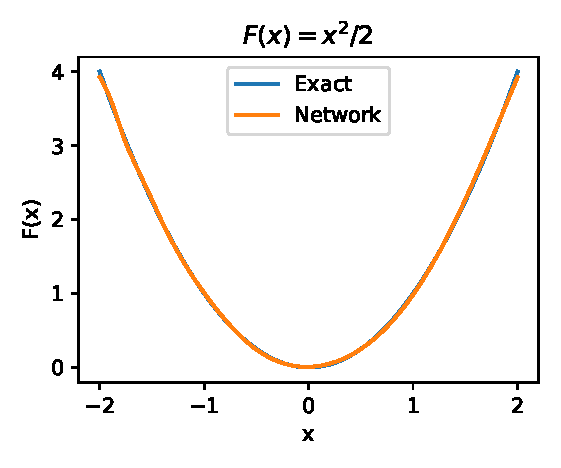
\includegraphics[width=.55\linewidth, trim={0 .2cm 0 .2cm}, clip]{1d.pdf}
    \caption{A trained network vs. exact $F(x)=\frac{1}{2}x^2$.}
    \label{fig:1d}
\end{figure}

We note that the endpoints of the function produced by the network are a bit off because there is less training data on the intervals closer to the endpoints.

\subsection{Test on the function $G$}
The hand-out suggested we use dimension $d=4$, and we can, to some extent, assert the same guesses as in for the function $F$. However, the training phase found that the values of $h$ and $\tau$ to be default or larger. Specifically, it admitted the quadruple $(10, 0.01, 4, 0.2)$, where the system converges when our measure of error is less than $10^{-4}$. Finally, the network produced the associated plot \autoref{fig:2d}.

\begin{figure}[h]
    \centering
    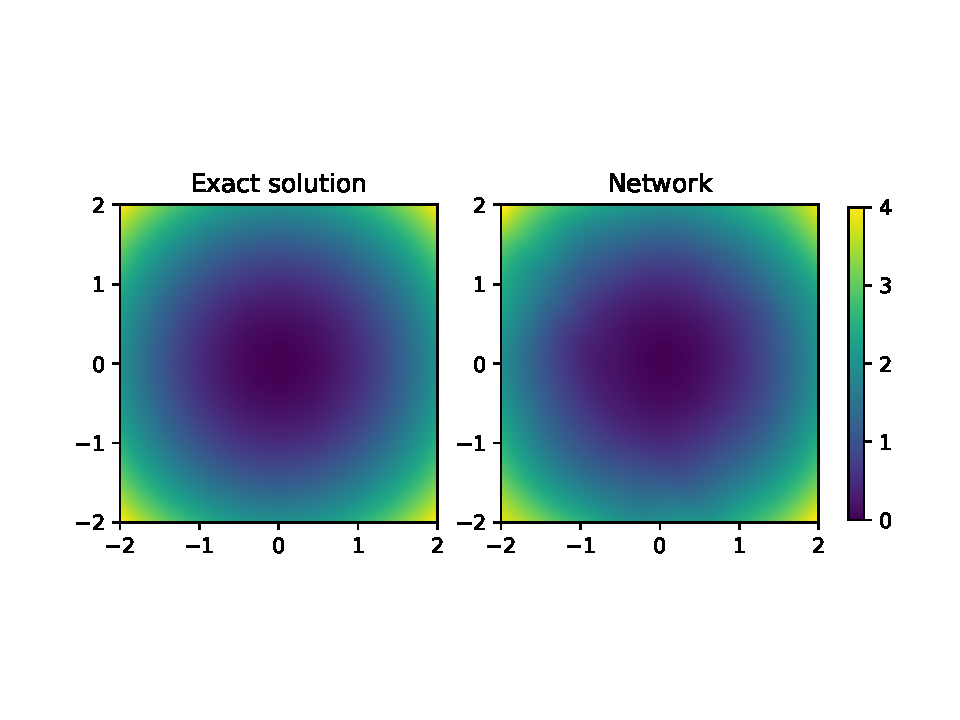
\includegraphics[width=\linewidth, trim={0 2cm 0 2.4cm}, clip]{2d.pdf}
    \caption{Comparison of the exact function $F(x_1,x_2)=\frac{1}{2}(x_1^2+x_2^2)$ versus a trained network.}
    \label{fig:2d}
\end{figure}

\section{Solving ODEs}
To solve dynamics in a Hamiltonian framework, one must solve the differential equations
\begin{align}
    \dot{q} &= \frac{\partial H}{\partial q} \label{eq:q} \\
    \dot p &= -\frac{\partial H}{\partial p}. \label{eq:p}
\end{align}
We know that methods with a symplectic property are preferred, which brings to mind the symplectic Euler method. However, the higher-order Størmer--Verlet method is better at preserving the constant energy along with the solutions, as seen in \autoref{fig:ode}. Additionally, it barely imposes a computational cost compared to the alternative. Hence, it was the chosen method for the problems. 
\begin{figure}[h]
    \centering
    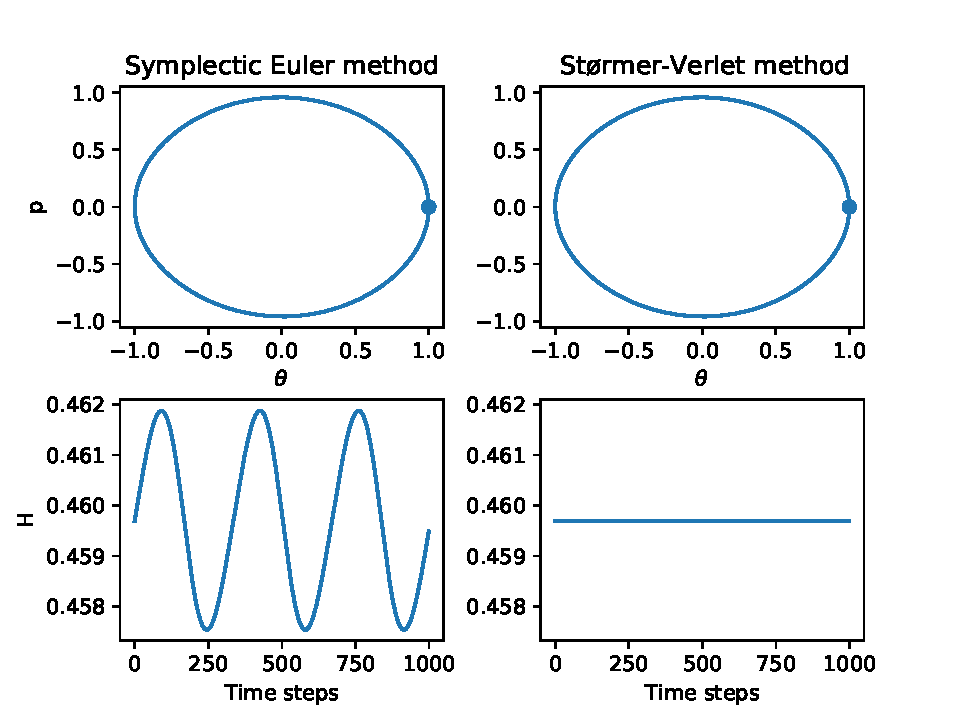
\includegraphics[width=0.8\linewidth]{ode.pdf}
    \caption{Comparison of the symplectic Euler method and the Størmer--Verlet method for a nonlinear pendulum.}
    \label{fig:ode}
\end{figure}

\subsection{Solving separable Hamiltonians}
For this section, we consider the nonlinear pendulum, which is given by the formula
\begin{equation}
    H(q, p) = \frac{1}{2} p^2 + mgl(1- \cos{q})
\end{equation}
where $q$ is the angle, $p$ the momentum, $m$ the mass, $g$ the gravitational acceleration and $l$ the pendulum length. Further, we chose the units such that $mgl = 1$. We use the network's \verb|grad| to solve the differential equations \eqref{eq:q}, and \eqref{eq:p}. A priori, we can guess the parameters will be similar to the test in \ref{eq:F} because the kinetic energy of the Hamiltonian is identical. The potential energy on the on an interval $[0,2\pi]$ also reassembles a parabola so we can make a similar a priori guess. 

The training phase admitted the quadruple $(6, 0.002, 2, 0.4)$ for both networks of the Hamiltonian, with convergence at $10^{-5}$. After feeding the network test data, we found the associated plot \autoref{fig:pendulum}, where we also computed the gradients of both networks.  
\begin{figure}[h!]
    \centering
    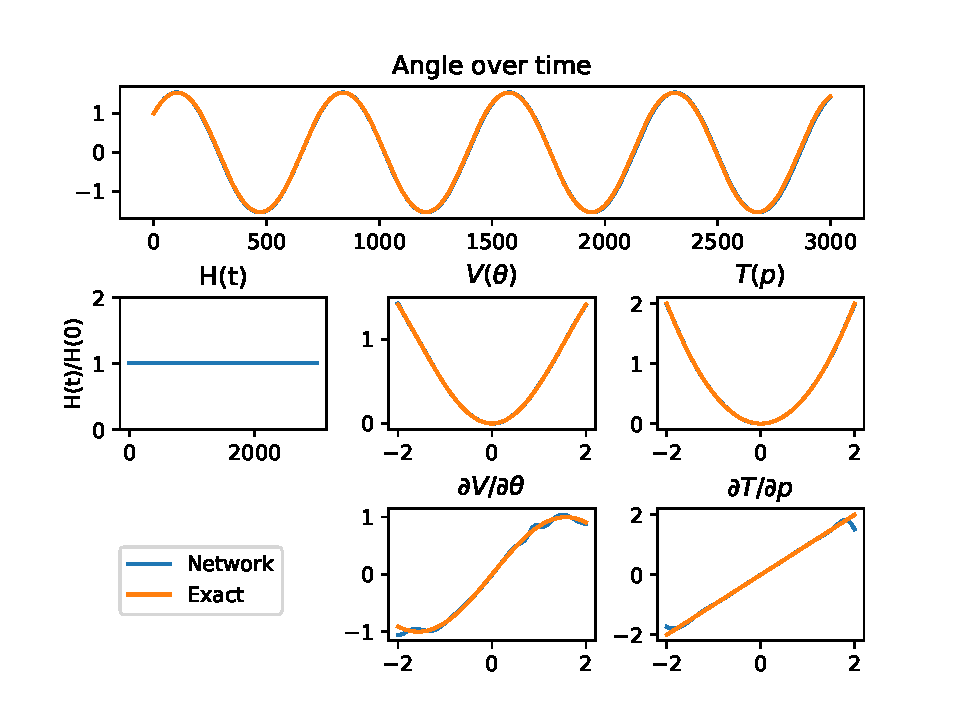
\includegraphics[width=\linewidth, trim={0 0.4cm 0 0.6cm}, clip]{pendulum.pdf}
    \caption{A nonlinear pendulum system solved using the Størmer--Verlet method with both the exact Hamiltonian function and a neural network.}
    \label{fig:pendulum}
\end{figure}

The exact solution and network's solutions are approximately identical, as implicitly predicted in our guess. The lack of training data constitutes some deviations on the interval between the network's - and the exact gradient. However, we note that the unfitness near the endpoints does not appear to cause any noticeable effect on the differential equation solution. Thence, the network can be trusted to compute the gradient of any finite system, by the the same arguments as in Section \ref{section 5}. 

\newpage
\section{Solving unknown Hamiltonian}
The inverse problem we are given can be summarised as follows: 
\begin{enumerate}
    \item We are given a large data set of time $t$, position $Q$, momentum $P$, kinetic energy $T$, and potential energy $V$.
    \item Train neural networks on this data.
    \item Compute the gradients of the trained functions.
    \item Solve dynamics in the Hamiltonian system.
    \item Compare solutions with given trajectories.
\end{enumerate}

\subsection{The given data}
Before we start training our network, we note that there are possible inconsistencies and inaccuracies in the given data. The function $V(q)$ appears to be exact but $T(p)$ does not share the same symmetry, as seen in Figure \ref{fig:given_data}. However, we can not definitively conclude that there is statistical noise in $T$. Yet, we are unable to conclude that $T$ is exact as we can with $V$. Although, we may be plotting $T(p)$ wrong and are thus unable to detect this error.

\begin{figure}[h]
    \centering
    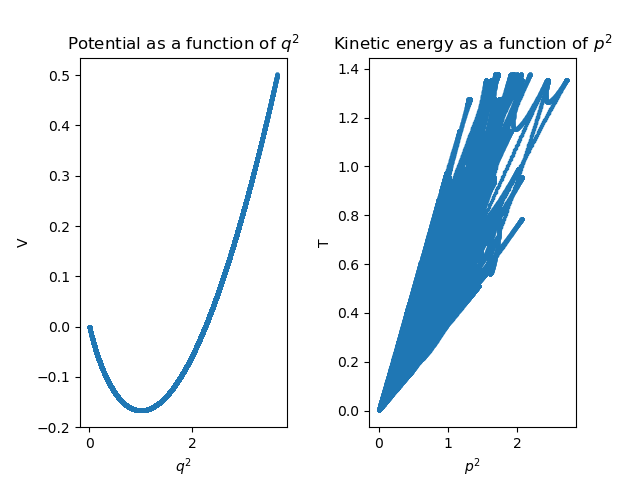
\includegraphics[width=\linewidth]{givendata.png}
    \caption{Visualisations of the complete set of given data.}
    \label{fig:given_data}
\end{figure}

\subsection{Training}
Ahead of the training phase, we could only make an a priori guess that because the data is has a high degree of complexity and possibly noise, that $K$ must be large and that $\tau$ and $h$ must be small enough to achieve a satisfactory degree of accuracy. The latter is especially important because this data set requires SGD. It is required because the data set is noticeably large ($\approx 200\,000$ data points). If we implement it into our training phase on this data, the required computation time will far exceed any extra accuracy achieved through the standard implementation used.

\begin{table}[h!]
    \centering
    \begin{tabular}{c|c}
        \textbf{Parameter} & \textbf{Value} \\
        \hline
         Batch size & 4096 \\
         $d$ & 6 \\
         $K$ & 32 \\
         $h$ & 0.05 \\
         $\tau_V$ & 0.002 \\
         $\tau_T$ & 0.01 \\
    \end{tabular}
    \caption{Parameters used for the networks when training on the unknown Hamiltonian.}
    \label{tab:parameters}
\end{table}

The parameters in \autoref{tab:parameters} gave adequate results within a reasonable time when training on the unknown trajectories. The network modeling $V(q)$ converged worse than $T(p)$ on the updated data. Thus, the learning parameter had to be lower and the iterations higher, as seen in \autoref{fig:error}. We ran the training process until the error measure reached $10^{-6}$, which in total, for both networks, required about 10 minutes on the machine used.

\begin{figure}[h!]
    \centering
    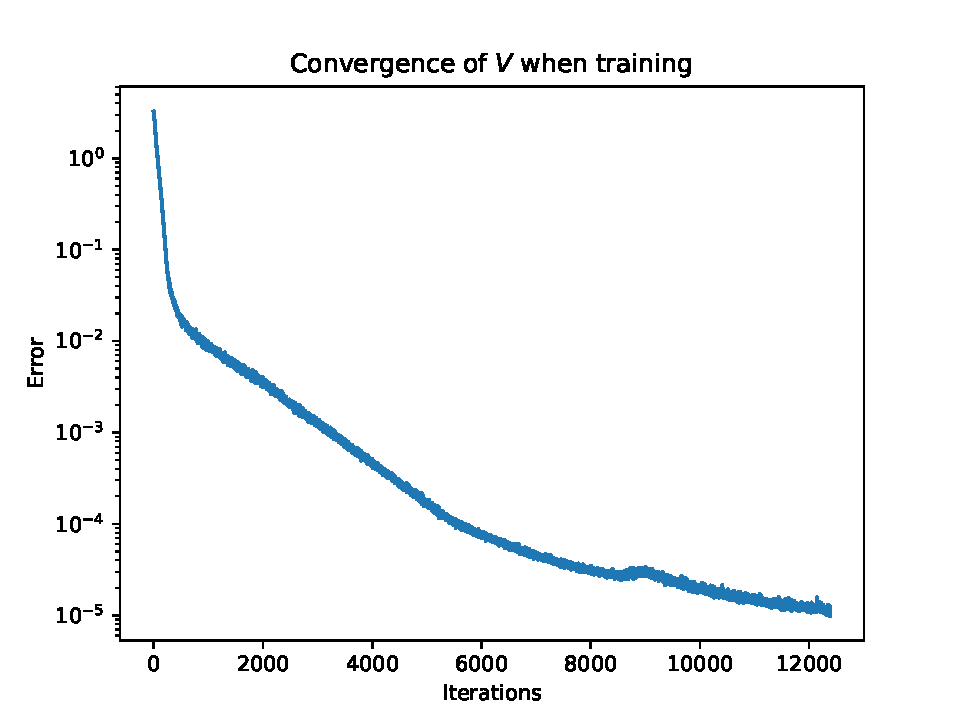
\includegraphics[width=.8\linewidth]{V_convergence.pdf}
    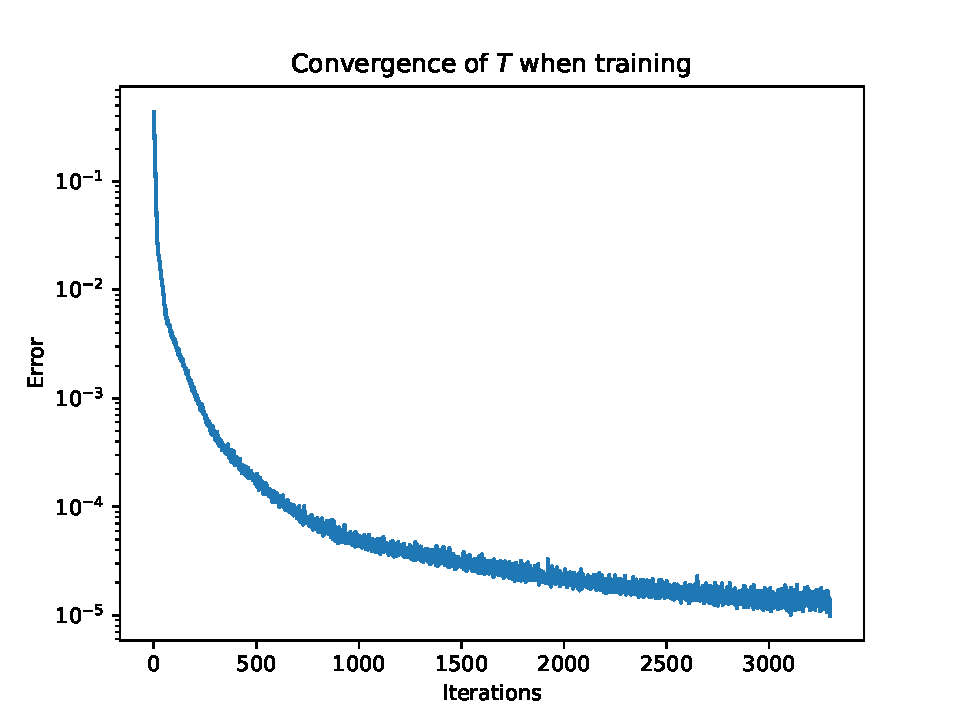
\includegraphics[width=.8\linewidth]{T_convergence.pdf}
    \caption{Network performances during training.}
    \label{fig:error}
\end{figure}

\subsection{Results}
After computing the gradients of the two networks, we solved dynamics in the unknown Hamiltonian system. \autoref{fig:ham_ode} shows a time propagation of the system calculated by using the Størmer--Verlet method on a trained network versus a given trajectory where both have equal initial conditions. Additionally, we show their Hamiltonians over time.

\begin{figure}[h!]
    \centering
    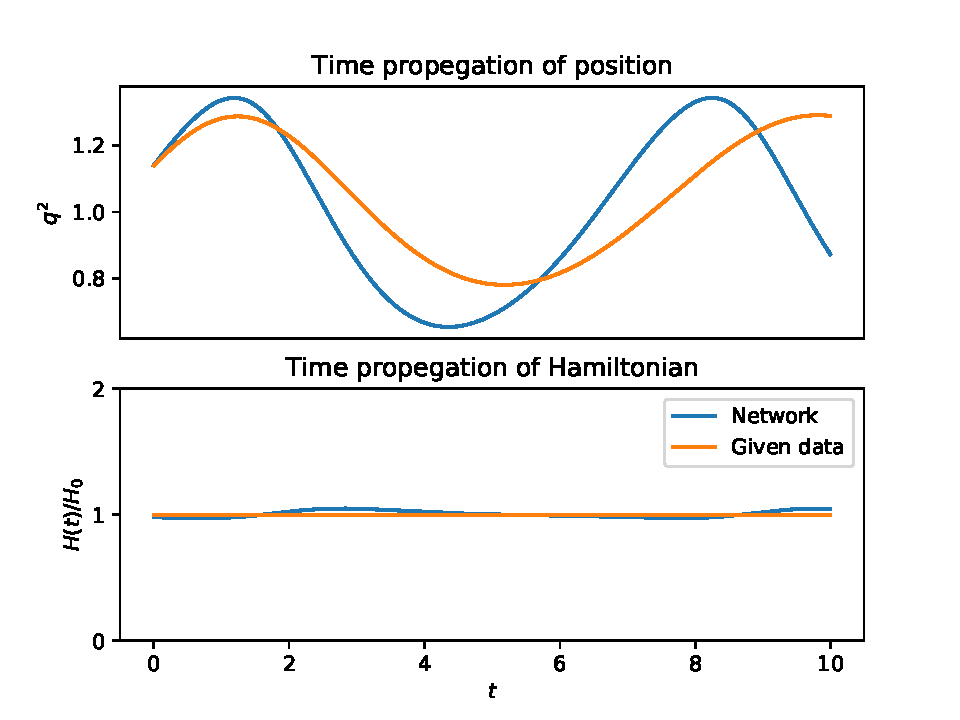
\includegraphics[width=\linewidth]{ham_ode.pdf}
    \caption{Hamiltonian dynamics solved with a trained network compared with a given trajectory.}
    \label{fig:ham_ode}
\end{figure}

The network does not precisely model the given trajectory, but it shares important similarities. The initial motion is similar, and the overall model follows the same general shape. The relative constancy of the Hamiltonian instills further trust in the model. The deviations are likely not due to an unknown problem in the neural network's method. However, it is likely due to insufficient convergence and computational limitations.

\section{Further development}
To develop our neural network further, we must first mention that the choices of our parameters would differ from our current parameters given unlimited time or computational power. In the real world, offloading the linear algebra to the GPU would drastically improve the overall performance. Increasing the number of layers, the number of internal dimensions and the batch sizes would overall improve our results. Similarly, decreasing our step-size and learning parameters would yield similar results. Another area of improvement is the general implementation. There might be inefficient array-conversions, memory allocations etc., which writing in a compiled language could remedy. 

\section{Conclusion}
This project implemented a neural network based on the ResNet architecture in \verb|Python|, which was successfully trained and tested on known data. This network was able to model an unknown Hamiltonian system, only using some given trajectories within the system as training data. The three-dimensional system had a higher degree of complexity and perhaps some data inaccuracies, and therefore, it did not achieve complete equality with the network and the given data. However, there is likely a more efficient implementation, and giving the system more computing time would provide better results.

\printbibliography
\end{document}
